\begin{flushright} {\tiny {\color{gray} app\_grading.tex}} \end{flushright}
%~~~~~~~~~~~~~~~~~~~~~~~~~~~~~~~~~~~~~~~~~~~~~~~~~~~~~~~~~~~~~~~~~~~~~~~~~~~~~~~~~~~~~~~~~~~~~~~~~~


\begin{itemize}
\item 
The document should contain your full name and student number on the first page. 
\item 
The file should be a pdf which name contains your family name
\item 
Layout: is the document visually pleasing? Is it well structured? 
\item Is there a complete bibliography (when applicable)?
\item Does the structure follows this: Introduction - Methods - Results - Discussion - Conclusion - Appendix ?
\item 
Figures: Are they properly numbered? captioned? all figures must be referenced in the text. 
Are they of good enough quality (no visible pixels)? are they readable? are all axis labelled?
\item 
Text: Overall quality of the language. Are there still typos? Do all sentence make sense?
\item if you wish to show lines of code, use verbatim or lstlisting\footnote{\url{https://en.wikibooks.org/wiki/LaTeX/Source_Code_Listings}} 
\item 
Discussion: are the results properly discussed, analyzed? are potential problems, errors, limitations discussed?
\item 
Conclusion: Are the findings/results summarized and generalized?
\end{itemize}

\begin{center}
\begin{tabular}{cc}
\hline
No & Yes \\
\hline
\hline
$6.67*10^{-11}$ & $6.67 \times 10^{-11}$ \\
$kg/m^3$ &  kg/m$^{3}$ or kg.m$^{-3}$\\
1x1 & 1$\times$1\\
$cos$ & $\cos$\\
docx file & pdf file \\
'if you do this'& passive form \\ 
\hline
\end{tabular}
\end{center}




%.....................................
\par\noindent\rule{\textwidth}{0.4pt}
\begin{center}
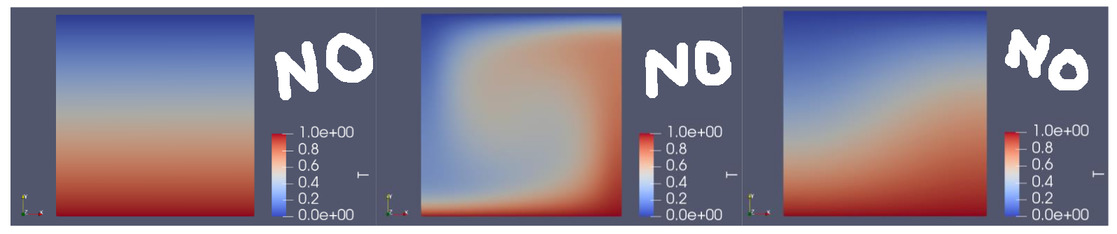
\includegraphics[width=10cm]{images/grading/grey}\\
No grey background
\end{center}


%.....................................
\par\noindent\rule{\textwidth}{0.4pt}
\begin{center}
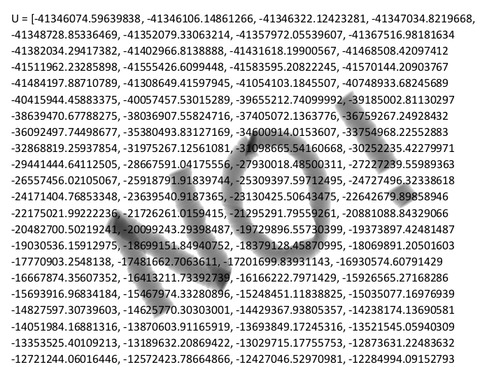
\includegraphics[width=8cm]{images/grading/numbers}\\
No lists/arrays with numbers
\end{center}

%.....................................
\par\noindent\rule{\textwidth}{0.4pt}
\begin{center}
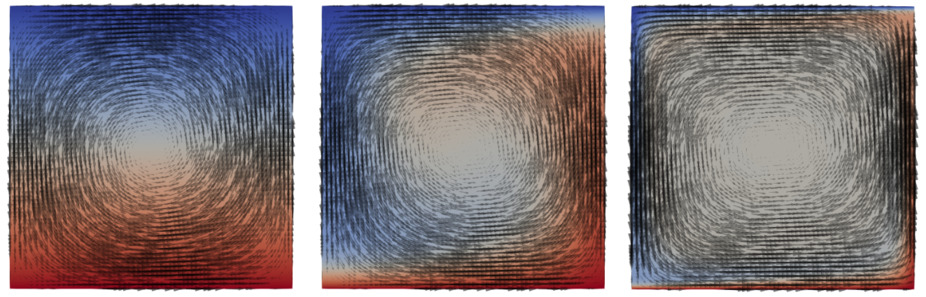
\includegraphics[width=10cm]{images/grading/arrows2}\\
Too many arrows\\
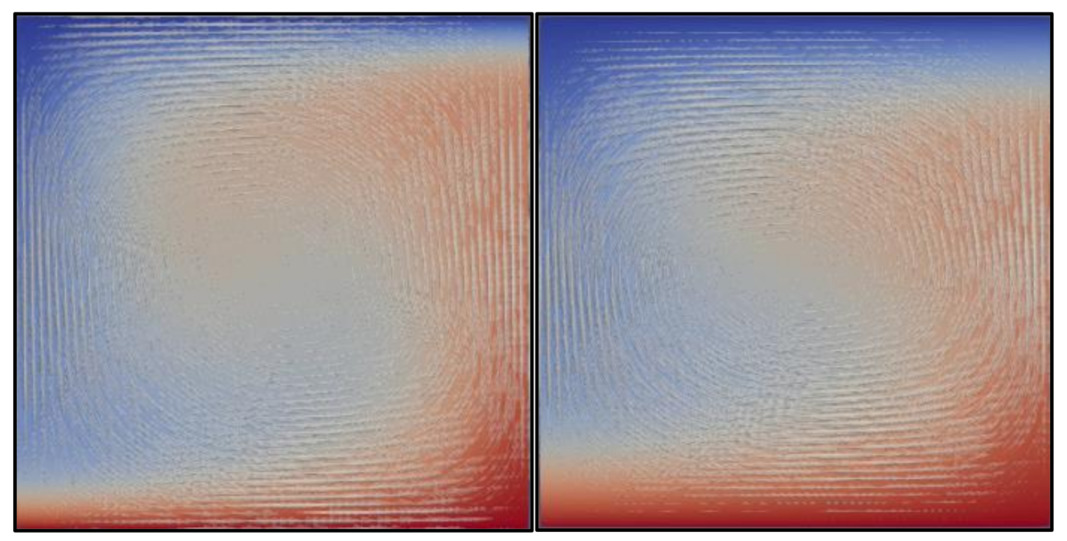
\includegraphics[width=9cm]{images/grading/arrows1}\\
Poor choice of arrow colour
\end{center}

%.....................................
\par\noindent\rule{\textwidth}{0.4pt}
\begin{center}
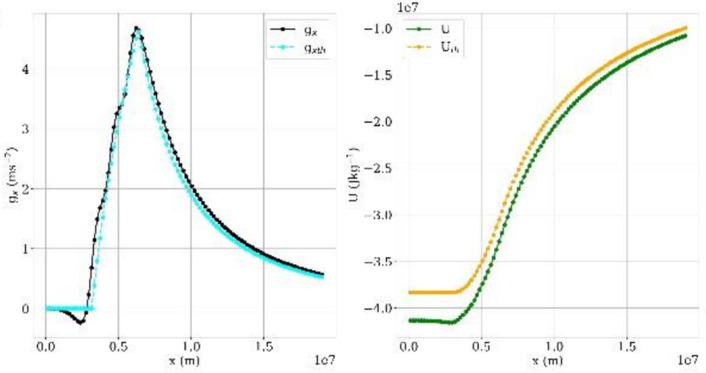
\includegraphics[width=8cm]{images/grading/pixels1}
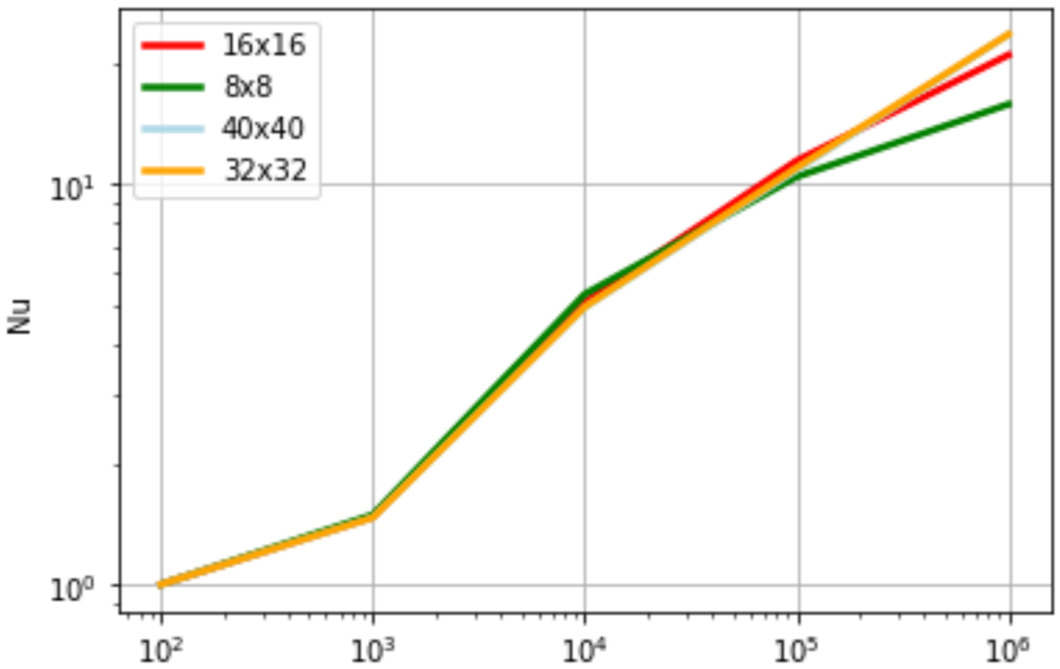
\includegraphics[width=7cm]{images/grading/pixels2}\\
Be careful about how you export your figures. These are unreadable.
\end{center}
 
%.....................................
\par\noindent\rule{\textwidth}{0.4pt}
\begin{center}
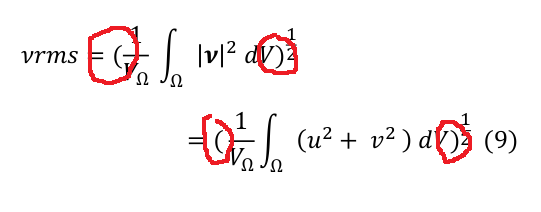
\includegraphics[width=8cm]{images/grading/eqs1}\\
Parenthesis too small
\end{center}

%.....................................
\par\noindent\rule{\textwidth}{0.4pt}
\begin{center}
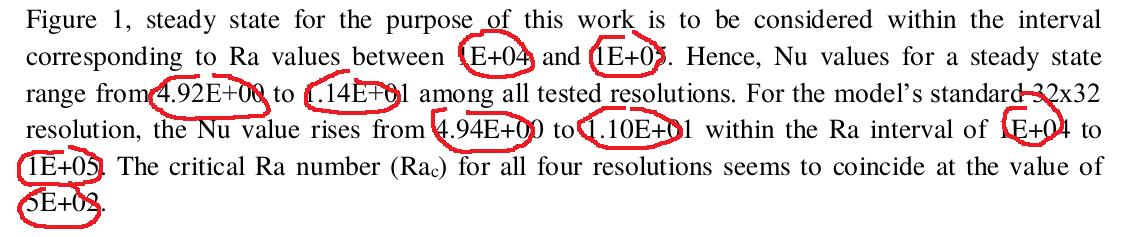
\includegraphics[width=9cm]{images/grading/eqs2}\\
1.6E+10 is not acceptable. Replace by $1.6\cdot 10^{10}$
\end{center}

%.....................................
\par\noindent\rule{\textwidth}{0.4pt}
\begin{center}
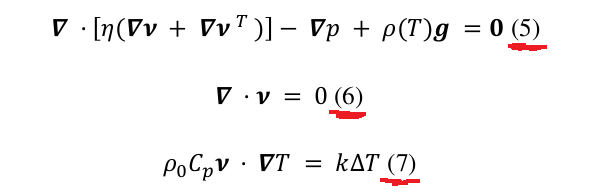
\includegraphics[width=7cm]{images/grading/eqs3}\\
Equation number is too close to the equation itself. Use labels, 
do not number equations by hand.
\end{center}

%.....................................
\par\noindent\rule{\textwidth}{0.4pt}
\begin{center}
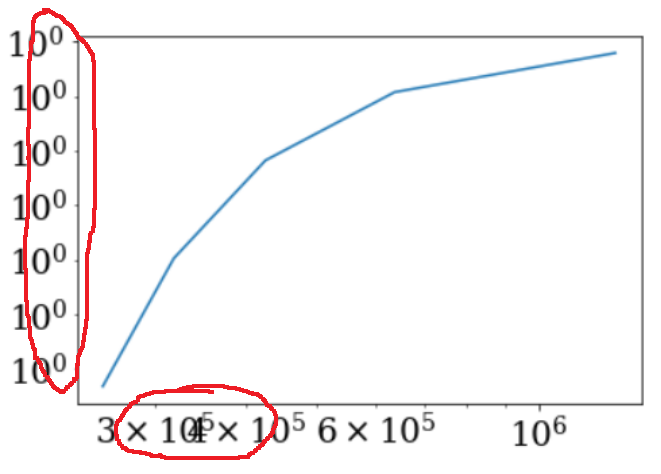
\includegraphics[width=9cm]{images/grading/eqs4}\\
Formatting of both axis lead to unreadable figure.
\end{center}

%.....................................
\par\noindent\rule{\textwidth}{0.4pt}
\begin{center}
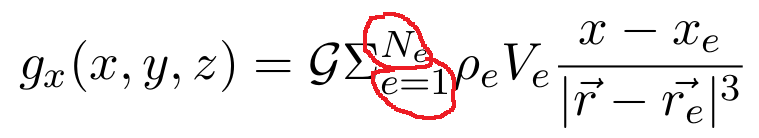
\includegraphics[width=9cm]{images/grading/eqs5}\\
In \LaTeX{}  use \verb!\sum\limits!
\end{center}

%.....................................
\par\noindent\rule{\textwidth}{0.4pt}
\begin{center}

\includegraphics[width=9cm]{images/grading/eqs6}\\
Are so many digits necessary?
\end{center}

%.....................................
\par\noindent\rule{\textwidth}{0.4pt}
\begin{center}
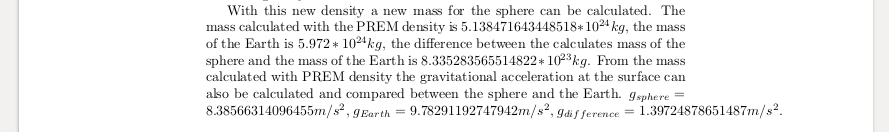
\includegraphics[width=10cm]{images/grading/width}\\
use \verb!\usepackage[cm]{fullpage}! to allow for wider text.
\end{center}

%.....................................
\par\noindent\rule{\textwidth}{0.4pt}
\begin{center}
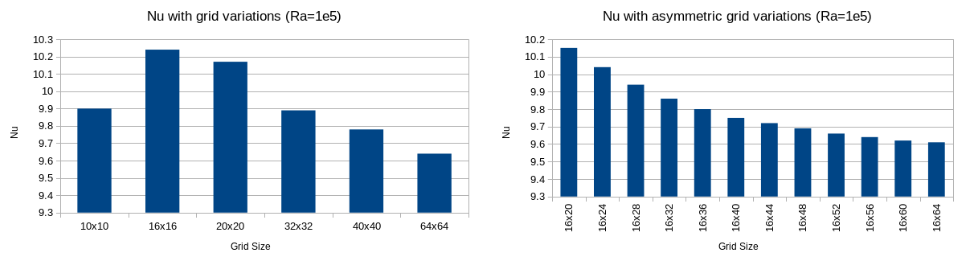
\includegraphics[width=10cm]{images/grading/figs1}\\
This figure style is to be avoided. Simply use dots and/or lines.
\end{center}

%.....................................
\par\noindent\rule{\textwidth}{0.4pt}
\begin{center}
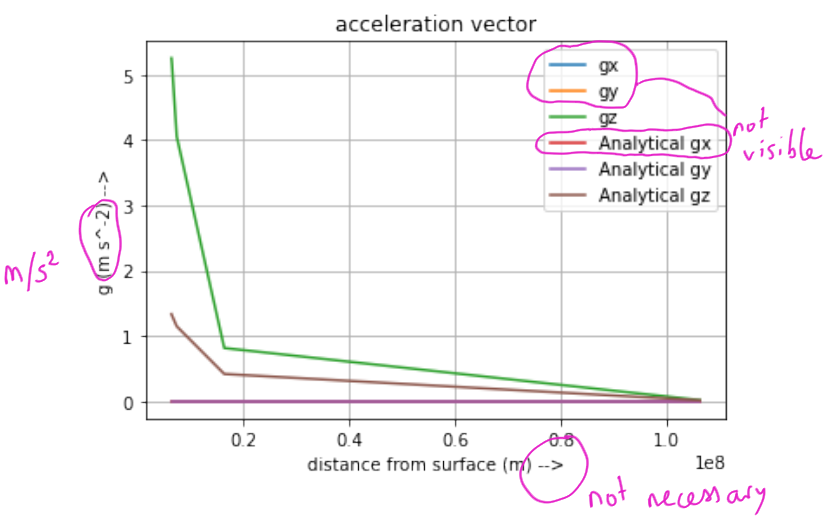
\includegraphics[width=8cm]{images/grading/figs2}
\end{center}

%------------------------------------------------------------
\subsection{Computational Geodynamics Report}

All the comments above apply, with additional instructions:
\begin{itemize}
\item report should be in \LaTeX 
\item The document should contain your full name and student number on the first page. 
\item The report file should be a pdf which name contains your family name
\item not more than 25 pages. If more, use appendices wisely.
\item document should be structured in two main parts: FDM and FEM.
\item no equations unless necessary to the discussion (still mention the equation that 
you are solving but refer to an external document/article/book for example).
\item use lstlisting package to include code
\item use {\verb| \usepackage[cm]{fullpage} |} to format your document
\item all codes either in appendix or in zip file (bearing your name).
\item a decent introduction (half page to one page) which links the topic of this course to geosciences.
\item discussion of results (stability, convergence, influence of resolution, remarks of all kinds).
\item if you did not succeed in doing a particular exercise, please explain what you think the problem is, 
how you know it is not working, etc ...
\item think about colormaps, image compression
\item DEADLINE: July 10th, 2022, 23:59 
\end{itemize}









